\chapter{Previous Work}\label{ch:prevwork}

The previous work I've completed has focused primarily on efforts to run and
benchmark simple, once-through fuel cycle simulations with \Cyclus. Supporting
this effort has required not only additions to the \Cyclus code base to model
enrichment and reactor facilities, but also to the peripheral (i.e., linking
and input/output) and simulation-related infrastructure.

Significant, strategic improvements have been added to the \Cyclus code base
regarding interactions with dynamically-loadable libraries and reading XML-input
files. Basic simulation setup and execution has been revised to provide clear
phases of initialization. Tools have also been added to provide agent-based
management of building and instantiation of child agents, i.e., facilities in the
\Cyclus simulation. A (currently) separate library, named \Cyclopts, has been
developed to provide an interface to optimization solvers which currently
supports COIN-OR's linear and integer program solvers
\cite{lougee_common_2003}. Management of the actual building (instantiation) of
facilities within the simulation framework has been encapsulated in a
supplier/manager class pair. Finally, additional support has been added
specifically regarding to model enrichment-related calculations, allowing for
enrichment facilities to be developed in \Cycamore.

The combination of the above enhancements, in addition to developing an
enrichment and batch-based reactor facility models, as well as a managerial
institution model and demand-based region model, resulted in a \Cyclus
once-through fuel cycle simulation. In order to benchmark the basic simulation
infrastructure, the INPRO \cite{_international_2009} once-through benchmark was
used and compared with results from the VISION \cite{yacout_vision_2006}
code. Output closely matched for both reactor growth, gross material flows, and
SWUs utilized. Discrepancies were seen for the amount of natural uranium
utilized. The exercise of developing an input file for the the benchmark
specification was tedious due to the lack of published specifications. After a
review of other benchmarks, this was shown to be a common problem in addition to
a general lack fully specifying benchmark scenarios. Accordingly, a new
specification language was proposed and implemented, and a translation package
was implemented in order to translate that input into a \Cyclus input file.

\section{\Cyclus To Date}

\subsection{Dynamic Loading}\label{sec:prev-dynamic}

Libraries can be accessed in a static manner, i.e., they are connected to an
application during the linkage phase, or can be accessed in a dynamic manner,
i.e., they are connected at run time. Dynamic linkage, or dynamic loading, is a
well-known technique for to support connectable, modular components, or
plug-ins. \Cyclus utilizes a plug-in approach for its facility, institution, and
region agents. This design decision furthers the \Cyclus development goal of
providing an agnostic framework into which sophisticated users can develop
different models of agents to investigate a certain simulation-modeling change.

Work was performed in order to use class-based representation of dynamic
libraries, allowing for easy opening, closing, and access thereof. Each dynamic
library represents an agent type in \Cyclus, providing a constructor and
destructor. The DynamicModule class then provides the \Cyclus Core access to
these constructors and destructors to perform the appropriate operations at run
time. Because dynamic loading is treated differently on POSIX-based systems than
it is on Windows-based systems, specialty functions for library access were
provided for each system. The correct header file (UnixHelperFunctions.h or
WindowsHelperFunctions.h) is chosen during compilation. 

These changes simplified the client code that utilizes library access. The
\Cyclus Core application can now call appropriate library-related functions in
an agnostic manner. Specific, well-defined time points of module loading
(dynamic library opening) and unloading (dynamic library closing) were defined
in the \Cyclus application. These operations, called by the application,
currently reside in the Model class and could likely be refactored into a
specific handler class designed for this purpose.

\subsection{Input Reading}

A large overhaul to the input-reading code base was performed. \Cyclus currently
only supports XML input files that adhere to the RNG schema defined in \Cyclus
RNG file. However, it is a well-known best practice to provide an agnostic
application programming interface (API) that can be configured with specific
instances given some user-defined input. Accordingly, such an API was
constructed which currently supports XML input but can also support future input
types that are tree-based (e.g., JSON, CSV, etc.).

The top-level abstraction is encased in a QueryEngine class. Basic operations
are provided assuming a tree-based input formation, including querying the
number of child elements at the current reading level, the name of each element,
and access to each element. The application code is responsible for configuring
the appropriate input parser and populating an instance of a QueryEngine at its
root. The client code then populates input parameters through the QueryEngine
interface rather than an input-format specific interface.

Support for XML-file reading has been enhanced by separating various concerns
into appropriate classes. Four classes have been constructed with specific
purposes regarding input file reading: file loading (XMLFileLoader), file
validation (RelaxNGValidator), file parsing (XMLParser), and querying
(XMLQueryEngine). The application interfaces with the file loader, initializing
it with a given input file path and then invoking the loading of various
\Cyclus-specific parameters (e.g., simulation control parameters, material
recipes, agent modules, etc.). The loader is responsible for managing its parser
and providing client code with correctly-configured instances of
XMLQueryEngines. The parser is responsible for providing an interface to the
underlying C++ XML parsing library (currently libxml++ is used) and invoking the
appropriate validation routines on the parsed file. The validator is responsible
for providing access to the RNG-validation operations through, currently, libxml
and libxml++. Finally, the XML-specific derived QueryEngine class is responsible
for implementing XML-specific querying using the generic QueryEngine interface.

Other input file formats can be supported by providing the appropriate
format-specific derived QueryEngine class and adjusting the application code as
necessary. To developer could then choose how to implement the loading and
validation, if any, of the input file. The above structure is just one of many
ways to achieve such a goal.

\subsection{Enrichment Tools}\label{sec:prev-enrich}

The ability to calculate enrichment-related values is required to provide
important metrics for the simplest of fuel cycle simulations. Enrichment is the
process of artificially increasing the relative amount of Uranium-235 in a given
sample of Uranium. Naturally, Uranium contains approximately 0.72\% U-235, a
small amount (~0.005\%) U-234, and 99.274\% U-238. In light-water reactors
(LWRs), fissile U-235 is the primary fission fuel source, and thus reactors run
longer with higher amounts of U-235. Accordingly, reactor fuels are enriched to
~3-6\% U-235. It should be noted that enrichment of Uranium above 20\% is
restricted by international law due to its capacity to be used as a weapon in
high concentrations. In practice, however, Uranium-based nuclear weapons
generally have enrichments of greater than 90\%.

The enrichment process has one input, or feed, stream (usually natural Uranium)
and two output streams, the product and the excess Uranium, called tails. The
U-235 abundance, or assay of each of these streams as well as the mass of each stream
determines how much work is required to perform the enrichment, where
enrichment-work is calculated using Separative Work Units (SWUs). The feed,
product, and tails stream mass and assay values are related. Equation
\ref{eqs:enr-feed} shows the relation between product and feed masses, and
Equation \ref{eqs:enr-tails} shows the relation between product and tails
masses. 

\begin{equation}\label{eqs:enr-feed}
  F = P \frac{x_{p} - x_{t}}{x_{f} - x_{t}}
\end{equation}

\begin{equation}\label{eqs:enr-tails}
  T = P \frac{x_{p} - x_{f}}{x_{f} - x_{t}}
\end{equation}

Note that both equations depend on the U-235 assay ($x_i$s) of each
stream. Furthermore, given the assay of each stream, one needs to either set
the product or feed value (in the case of Equation \ref{eqs:enr-feed}) and the
product or tails value (in the case of Equation \ref{eqs:enr-tails}). In
practice, the feed and tail assays are set and an order for some quantity of
enriched product is requested. The resulting required feed and tail masses are
then calculated.

Enrichment plants measure their production in SWUs due to the quality
(enrichment level) variation of their product from order to order. The amount of
SWUs required to enrich a quantity of Uranium to a certain assay is a
function of all of the aforementioned variables (assays and masses of the
feed, product, and tails streams). The SWU calculation is shown in Equation
\ref{eqs:enr-swu}, where $V(x)$ is the Value Funtion defined in Equation
\ref{eqs:enr-value}.

\begin{equation}\label{eqs:enr-swu}
  SWU = P \; V(x_{p}) + T \; V(x_{t}) - F \; V(x_{f})
\end{equation}

\begin{equation}\label{eqs:enr-value}
  V(x) = (1 - 2x) \ln \left( \frac{1-x}{x} \right)
\end{equation}

Combining Equations \ref{eqs:enr-feed}, \ref{eqs:enr-tails}, and
\ref{eqs:enr-swu}, one can represent the SWU calculation as a function only of
the product mass and feed, product, and feed stream assays as shown in
Equation \ref{eqs:enr-swu-p}.

\begin{equation}\label{eqs:enr-swu-p}
  SWU = P \left( V(x_{p}) + \frac{x_{p} - x_{f}}{x_{f} - x_{t}} V(x_{t}) 
        - \frac{x_{p} - x_{t}}{x_{f} - x_{t}} V(x_{f}) \right)
\end{equation}

An Enrichment class was added to the \Cyclus set of utility toolkits under the
enrichment namespace. A simple Assay container class was also added, and is used
as the argument to many of the above calculations. The Enrichment toolkit allows
for the calculation of each of the abovementioned values and is used primarily
in the EnrichmentFacility that was added to \Cycamore to run the once-through
fuel cycle benchmarks.

\subsection{Facility Building and Supply/Demand Tools}

In order to support simple, once-through fuel cycle simulations, a nominal
capacity supply-demand interaction capability was needed. The use case of such a
system is to define demand for a given installed capacity, say in gigawatts of
produced power. Agents in a \Cyclus simulation generally have a natural
life cycle, leaving the simulation at the end of their lifetimes. The system must
be able to respond to changes in installed capacities if it is to continue to
meet the simulated demand curves.

\subsubsection{Facilities as Prototypes}
After reviewing the prior status of the code base and the way in which
Facilities were being defined and instantiated, I noted that there was not a
well-formed entry or exit point for facilities in the simulation
infrastructure. Accordingly, I updated the methodology behind such operations to
use the Prototype design pattern \cite{vlissides_design_1995}. A prototype is a
creational pattern that keeps a prototypical instance of an object
available. When a new instance is required, a copy of this prototypical instance
is made and returned. This strategy fit naturally with the \Cyclus input format
and code base. Nominal parameters defining ``classes'' of facilities, e.g., a
certain type of reactor or supporting facility, are listed in XML input
files. The code base has been updated to create prototypical instances of each
facility defined in the input file during a simulation initialization step. When
a new facility is required to be built in the simulation, a copy of a prototype
is introduced.

\subsubsection{Symbolic Functions}

The ability to represent symbolic functions was added to the \Cyclus Utility
toolkit. Functions are represented by a base Function class providing an
appropriate API. Linear, exponential, and piece-wise function classes are
supported, where piece-wise functions can utilize both linear and exponential
piece-wise functions. Factory classes are provided to take a string of parameters
as read from an input file and return the appropriate symbolic function. A
simple example of the piece-wise function support is provided in Figure
\ref{fig:piecewise}.

\begin{figure}[H]
  \begin{center}
    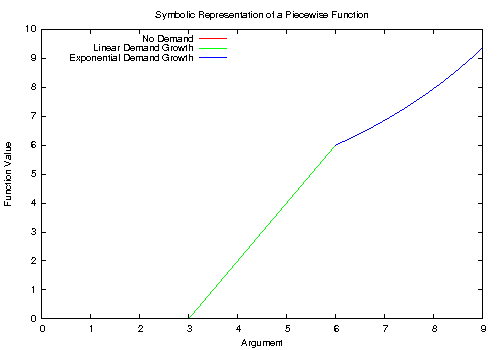
\includegraphics[width=\linewidth]{./chapters/prevwork/piecewise.png}
  \caption{An example of a piece-wise function represented using the updated API.}
  \label{fig:piecewise}
  \end{center}
\end{figure}

\subsubsection{Tracking Commodity Production Capacity}

There is a need to track the current capacity of the production of a certain
commodity. Electrical power was offered as the prime example for this
once-through fuel cycle use case. Accordingly, a simple ``mixin'' class
\cite{ulrich_mixin-based_2001} called CommodityProducer was developed. It offers
an interface for accessing a list of commodities an entity produces and their
associated capacity to produce each commodity as well as the unit price of
commodity production. To date, the mixin has been used in conjunction with the
BatchReactor class, which serves as the reactor model for the once-through fuel
cycle simulations. The BatchReactor subclasses from both the base Facility class
as well as the CommodityProducer class.

A CommodityProducerManager class was also developed to manage a collection of
commodity producers. Its interface include registration and unregistration
methods to keep track of the producers it manages as well as a simple interface
for querying the current total capacity level of the commodity producers it
manages. It is also designed as a ``mixin'' class which has been utilized by the
ManagerInst class in \Cycamore, allowing the institution to keep track of the
capacity of facilities that produce certain commodities (e.g., electrical
power). This manager class is a use of the classic Observer design pattern
\cite{vlissides_design_1995}.

\subsubsection{Supply/Demand Tracking and Intelligent Build Decisions}

Three concerns remain in order to implement an appropriate model of responses to
changing supply capacity and demand for capacity. First, the current supply and
demand levels must be query-able. Second, if demand is greater than supply, some
new simulation entity must be built or introduced into the simulation. Third, a
decision must be made as to which entities should be built to meet a demand gap
if it exists.

A SupplyDemandManager class has been introduced to provide an interface for
querying the current supply capacity and demand for a given commodity. The class
is an Observer of CommodityProducerManagers, querying them when appropriate to
determine the full production capacity for the union of CommodityProducers
managed by the set of CommodityProducerManagers. Demand functions are also
registered for each commodity. An instance of a SupplyDemandManager is a private
member of the GrowthRegion class in \Cycamore, which supports building
facilities based on user-defined growth curves.

A Builder class has been introduced an interface for an entity that can build,
or instantiate into the simulation, instances of CommodityProducers. It is
designed as a ``mixin'' class and is utilized by the ManagerInst class in
\Cycamore. To date, institutions have been thought of as managers of facilities
by the \Cyclus development team, thus it is possible that the notion of facility
deployment management encapsulated in the current version of the ManagerInst
could be refactored into the Institution base class in the \Cyclus core
database. Such a decision will be informed by present and future use cases.

Finally, the BuilderManager class has been introduced to encapsulate the
decision making operations regarding building new facilities. It is an Observer
of Builder class instances, and an instance of the BuilderManager is used as a
private member by the GrowthRegion class in \Cycamore. The BuilderManager
interacts with the region's SupplyDemandManager to query the existence of unmet
demand. If it exists, it solves an integer program formulated as Equation
\ref{eqs:build-decision},

%%% 
\begin{subequations}\label{eqs:build-decision}
  \begin{align}
    %%
    \min \:\: & 
    \sum_{f \in F} n_f c_f
    & \\
    %%
    \text{s.t.} \:\: &
    \sum_{f \in F} n_f \phi_f \ge \Phi
    & \\
    %%
    &
    n_f > 0 \: \text{and} \: integer
    &
    \forall f \in F
    %%
  \end{align}
\end{subequations}
%%% 
  
where $\Phi$ is the unmet demand, $F$ is the set of facilities capable of
meeting the demand, and, for each facility in $F$, $c_f$ is the cost of
building, and $\phi_f$ is the nameplate capacity.  Finally, $n_f$ is the
optimized number of facilities to build of type $f$. The set of facilities and
their associated costs and capacities are queried through the managed Builder
instances.

\subsection{\Cyclopts}

Proposed in this thesis and already implemented in the \Cyclus code base is a
heavy usage of integer and linear programming. The domain of mathematical
programming is well studied and many LP, IP, MILP solvers exist. The majority of
solvers or codes supporting such solvers are closed source (e.g., BARON, CPLEX,
Maple, MATLAB, etc.). Such programs are generally faster than their open source
cousins, but are restrictive to use in implementation of an open source library
like \Cyclus. Accordingly, there is a use case for providing an abstract
interface for defining mathematical programs that can support concrete
implementations based on the library used.

\Cyclopts has been developed as a separate library to provide such an
interface. Basic constructs such as variables, functions, and solvers are all
represented as concrete classes. Different solver libraries are implemented by
deriving from the base Solver class. An interface class is provided to connect
abstract concepts required to define a problem instance with a concrete solver.

Currently, COIN-OR's Coin-Branch-and-Cut (CBC) \cite{lougee_common_2003} solver
is supported as a proof of principle. The \Cyclopts library is used by the
BuilderManager class in \Cyclus to determine the solution of Equation
\ref{eqs:build-decision}. Future development will include adding a full test
suite to \Cyclopts and integrating it as a part of the \Cyclus core as
additional use cases present themselves. Such cases will arise through the
implementation of this thesis.

\section{Benchmarking Efforts}\label{sec:prev-benchmark}

As with any code base, validation and verification (V \& V) exercises are
critical to have confidence in the answers provided by the code. Fuel cycle
simulators are an interesting V\&V case in that they model proposed future cases
of nuclear fuel cycles, rather than modeling physical systems that can, in some
part, be precisely experimentally-verifiable. Accordingly, predefined scenarios
are generally used to compare different codes to determine relative differences
between them. A number of benchmarking efforts exist with varying degrees of
documentation, one of which is the INPRO benchmark - the target of a comparison
between \Cyclus and VISION for once-through fuel cycle cases. During this
exercise and in conjunction with investigating expanding the benchmark scope, a
potential deficiency was discovered. Very rarely do benchmarks describe in
single location a concise summary of the parameters used therein. In some cases,
parameters are missing, and in others they are simply no provided to the
public. Accordingly, a new process for forming and disseminating benchmarks was
proposed and a proof-of-principle example was developed.

\subsection{Benchmarks of Once-Through Fuel Cycles vs. VISION}

The \Cyclus core and \Cycamore modules were used to conduct a benchmark
comparison with VISION, a fuel cycle code developed in PowerSim and Excel by the
Idaho National Laboratory. A single case was compared, the INPRO GAINS
\cite{_international_2009} once-through fuel cycle case. The specific reactor
and fuel parameters were communicated to the research group by personal email of
one of the participants at the IAEA \cite{dixon_re:_2009}.

% growth
\begin{figure}[ht]
  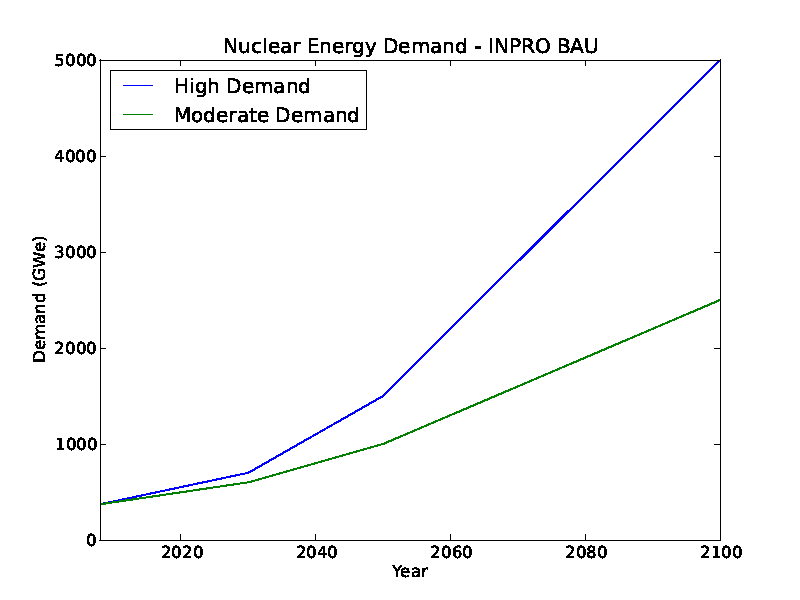
\includegraphics[width=\linewidth]{./chapters/prevwork/graphs/inpro-demand.png}
  \caption{Electricity demand in each INPRO demand case.}
  \label{fig:inpro-demand}
\end{figure}

The benchmark specified two growth scenarios, moderate and high, as shown in
Figure \ref{fig:inpro-demand}. Electricity growth was to be met mostly by PWR
reactors (94\%) with the remaining amount being met by HWR reactors (6\%). The
major metrics submitted for comparison in the INPRO GAINS work were deployment
curves and gross material flows. VISION also has the ability to output many
other metrics, of which enrichment-related parameters, i.e., natural uranium
usage and SWU consumption, were compared in this case.

Reactor deployment curves are shown in Figure \ref{fig:rxtrs}. General agreement
is met between the two codes, with a slight difference occurring in how the first
time step is handled with regard to output recording between the two. There is
no difference from a system dynamics or simulation mechanics point of view. 

% reactors
\begin{figure}[ht]
  \centering
  \subfloat[Low Case]{%
    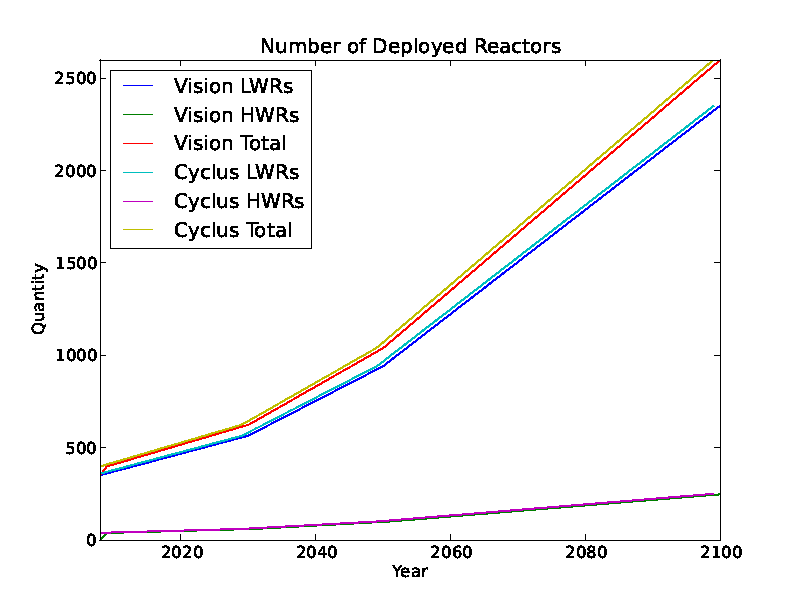
\includegraphics[width=.45\linewidth]{./chapters/prevwork/graphs/rxtrs_low.png}
    \label{fig:rxtrs_low}}
  \quad
  \subfloat[High Case]{%
    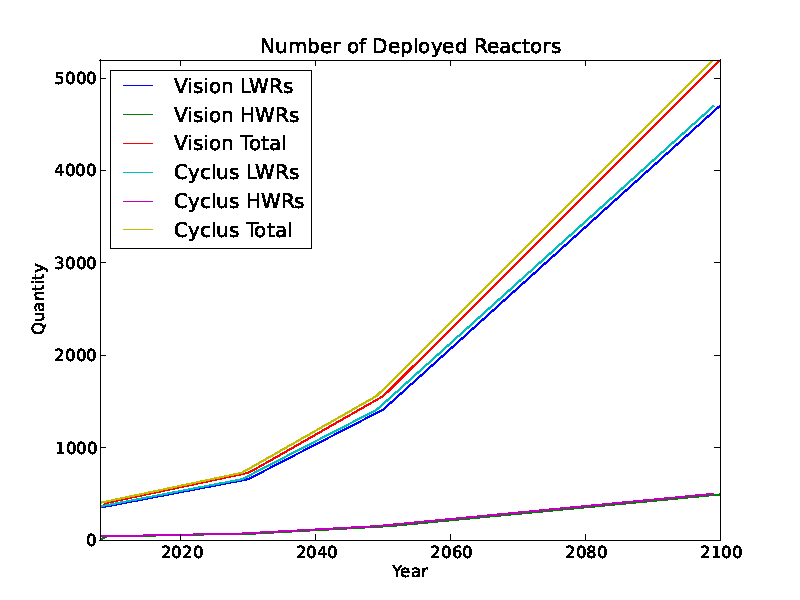
\includegraphics[width=.45\linewidth]{./chapters/prevwork/graphs/rxtrs_high.png}
    \label{fig:rxtrs_high}}
\caption{Reactors built in each INPRO demand case.}
\label{fig:rxtrs}
\end{figure}

VISION outputs fuel mass flow curves on a cumulative basis, i.e., a report for
some time t includes the flows occurring at time t plus all flows occurring at
previous times. Accordingly, a slight discrepancy, occurring at each time period,
compounds the error as time increases using such a metric. This phenomenon is
seen in Figure \ref{fig:used_fuel} with respect to the material flow of used
fuel out of reactors. A hand calculation of the flow for the first year time
step confirmed that the \Cyclus results were correct given the parameters
provided. The small difference, consistent between moderate and high scenarios,
becomes compounded with time. 

% used fuel
\begin{figure}[ht]
  \centering
  \subfloat[Low Case]{%
    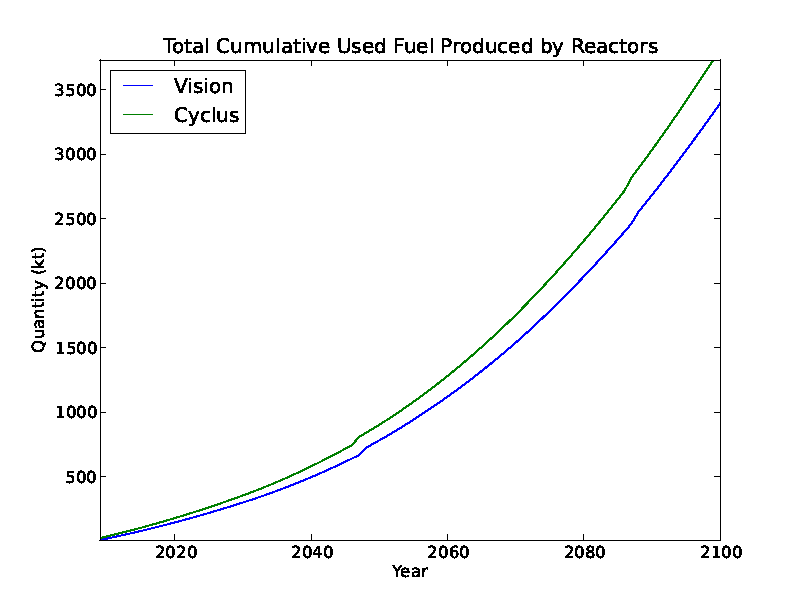
\includegraphics[width=.45\linewidth]{./chapters/prevwork/graphs/used_fuel_low.png}
    \label{fig:used_fuel_low}}
  \quad
  \subfloat[High Case]{%
    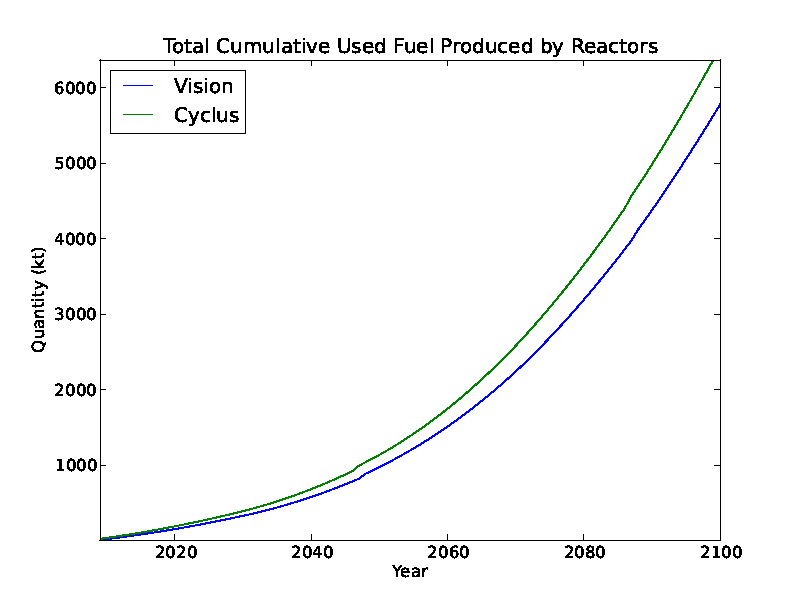
\includegraphics[width=.45\linewidth]{./chapters/prevwork/graphs/used_fuel_high.png}
    \label{fig:used_fuel_high}}
\caption{Used fuel exiting reactors in each INPRO demand case.}
\label{fig:used_fuel}
\end{figure}

VISION provides two enrichment-specific parameters as output metrics: cumulative
natural uranium used each year and cumulative SWUs consumed each year. Each of
these was compared for both demand scenarios. The results of the natural uranium
consumption comparison is shown in Figure \ref{fig:nat_u}, showing quite good
comparisons between the two codes in this regard. There exists a small
discrepancy related to the first time period phase shift with respect to
reporting differences between the two codes, as was also seen in Figure
\ref{fig:rxtrs}. The results comparing SWU values shown in Figure \ref{fig:swu}
are markedly different. It is not clear why VISION reports such a dramatically
different set of values, given that the amount of SWUs is directly related to
the amount of natural uranium used and the amount of fuel produced, two metrics
already shown to be quite close. Because SWU usage is an analytical calculation
given fuel input and output requirements, the \Cyclus values were checked by
hand for the first time steps and shown to be in accordance with expectations.

% nat u
\begin{figure}[ht]
  \centering
  \subfloat[Low Case]{%
    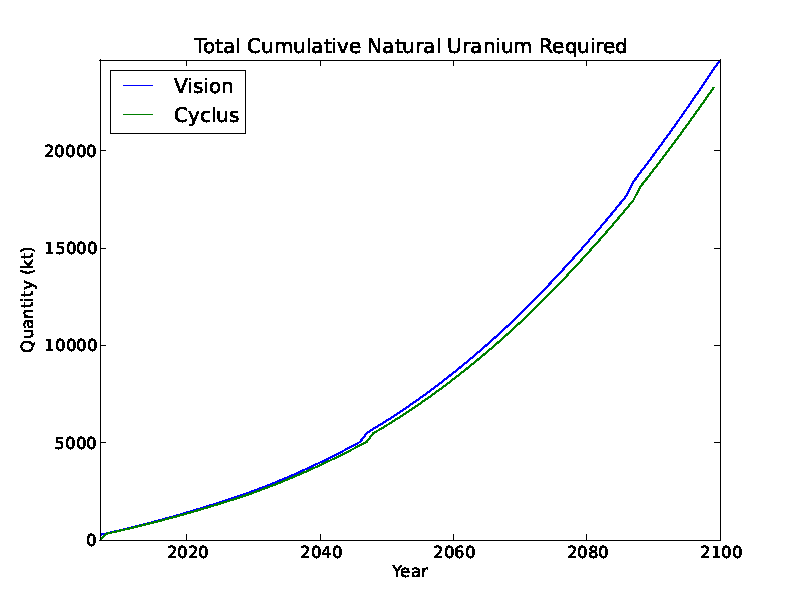
\includegraphics[width=.45\linewidth]{./chapters/prevwork/graphs/nat_u_low.png}
    \label{fig:nat_u_low}}
  \quad
  \subfloat[High Case]{%
    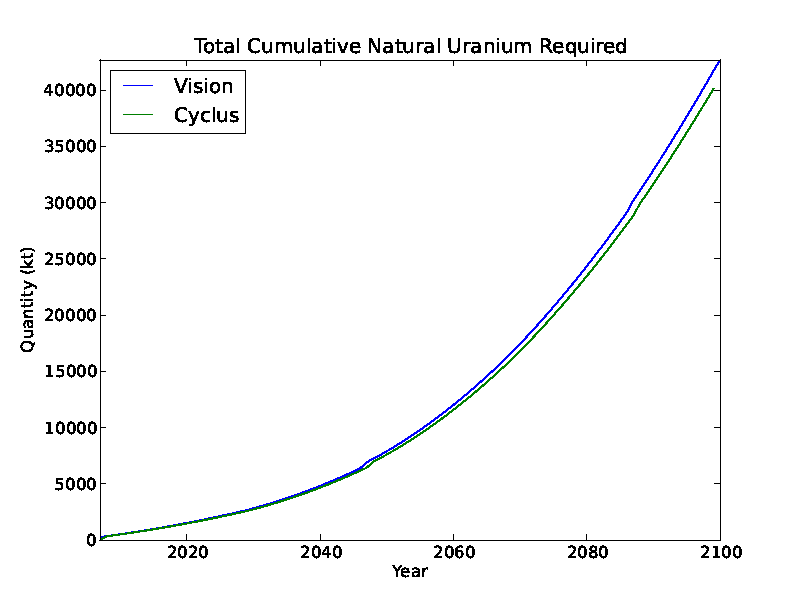
\includegraphics[width=.45\linewidth]{./chapters/prevwork/graphs/nat_u_high.png}
    \label{fig:nat_u_high}}
\caption{Natural uranium usage in each INPRO demand case.}
\label{fig:nat_u}
\end{figure}

% swu
\begin{figure}[ht]
  \centering
  \subfloat[Low Case]{%
    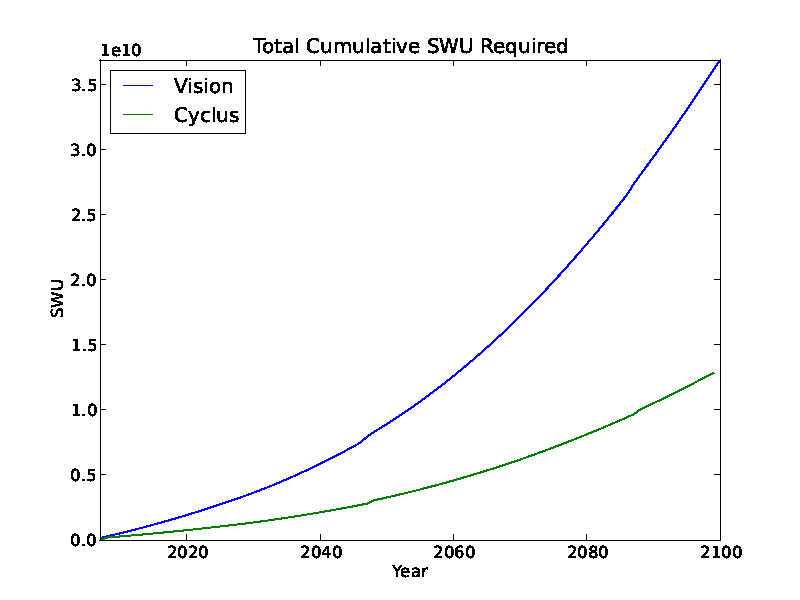
\includegraphics[width=.45\linewidth]{./chapters/prevwork/graphs/swu_low.png}
    \label{fig:swu_low}}
  \quad
  \subfloat[High Case]{%
    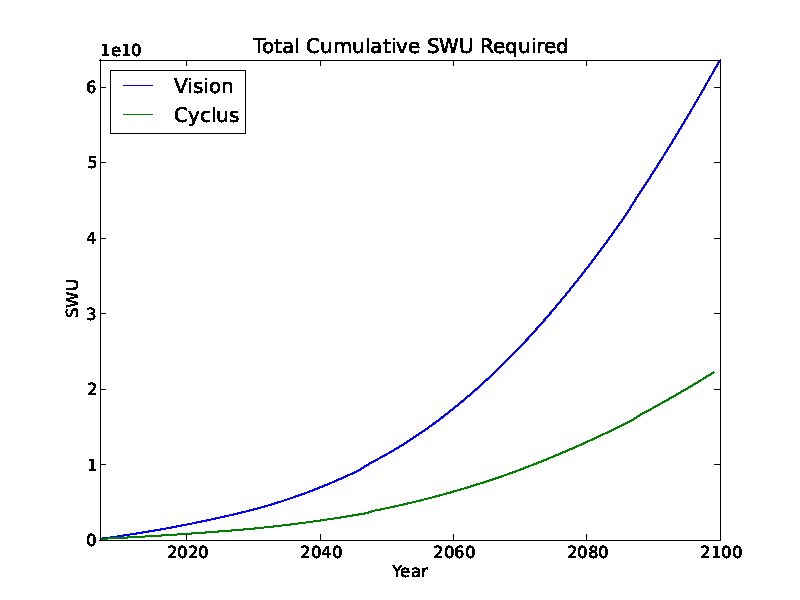
\includegraphics[width=.45\linewidth]{./chapters/prevwork/graphs/swu_high.png}
    \label{fig:swu_high}}
\caption{SWU usage in each INPRO demand case.}
\label{fig:swu}
\end{figure}

VISION and \Cyclus mostly agree with each other regarding the core output
metrics of reactor deployment and used fuel production in this simple
case. Significant questions remain regarding the difference in SWU consumption,
which can be addressed with the VISION team if further development of VISION is
pursued. A full description of the work was presented at the 2012
ANS Winter conference \cite{gidden_once-through_2012}.

\subsection{Benchmark Specification Language}

There have been a number of different benchmarking exercises attempted by
governmental and international agencies including the International Atomic
Energy Agency (IAEA) \cite{_international_2011} and the Nuclear Waste Technology
Review Board (NWTRB) \cite{_nuclear_2011}.  Both examples formulated their
benchmark specifications at meetings involving all participants, but have not
provided the full specifications to the public realm. MIT coordinated a
benchmarking exercise for dynamic simulators of advanced fuel cycles (i.e., fast
reactors with different conversion ratios) \cite{guerin_benchmark_2009},
including a specification with higher fidelity than those above. The
Organization for Economic Cooperation and Development (OECD) has also led a
benchmarking exercise that covers an example each of open, modified open, and
closed fuel cycles \cite{boucher_benchmark_2012} and provided a more detailed
specification \cite{boucher_specification_2008}.

Ubiquitous amongst all of the above-mentioned benchmarks is a lack of a common
language to describe scenario specifications. Once set, a given specification is
generally included as prose and numeric tables in a final report, and it may not
include all the required information to perform the benchmark
calculation. Accordingly, developing a specification language would greatly
benefit the fuel cycle simulation community by allowing for a common and
well-defined set of scenario parameters to be discussed. An example from the
nuclear data community is the push towards Generalized Nuclear Data (GND)
\cite{mattoon_generalized_2012}. This language is a \emph{specification} rather
than an \emph{implementation}, allowing others to tailor implementation details
(e.g., via XML, HDF5, etc.) to their needs.

Recognizing a lack of a common definition, work was performed to develop a
proof-of-principle language which can describe fuel cycle simulation scenario
benchmarks. A translation package was then written to translate the prototype
language into \Cyclus input. Finally, the translated \Cyclus input was used to
run the same INPRO GAINS benchmark above. An overview of the specification
language follows below. A full description of the work was presented at the 2013
ANS Summer conference \cite{gidden_developing_2013}.

\subsubsection{Materials}
Materials in a fuel cycle simulation generally come in two flavors: specified
recipes, which are normally defined as input for reactors, and the resulting
output which is a function of the input and applied burnup. We denote the two
flavors as being recipes or not. To begin, all material types are tagged by a
given name. Recipes are currently the application of a rigid definition of
constraints. There are hard-coded concentration values for each isotope in the
recipe as well as a static density value. Because the output is a result of a
physics calculation which may be implemented with varying fidelity, a less rigid
approach is used for non-recipes. The specification does not explicitly name all
isotopes in the output fuel. Rather it defines more liberal constraints on
certain isotopes that are physically provable.  (For example, a constraint may be
phrased as ``the concentration of species X must lie between concentrations A
and B.'') Lastly, we provide a parent field which takes as an argument another
material. This is a short-hand way of denoting trees of materials, i.e.,
multiple materials with mutual constraints. An example is provided in
Figure~\ref{fig:material}.

\begin{figure}[h!]
\begin{Verbatim}[frame=single]
"materials": {
  "nea_leu": {
    "recipe": true,
    "attributes" : {
    "concentrations": ["float","atom"],
    "density": ["float","g/cc"]
   },
   "constraints": [        
     ["U235", 0.0495],
     ["U238", 0.9505],
     ["O16", 2.0],
     ["density", 10.2]
   ], 
   "parents": []
  },
  "nea_spent_pwr_uox": {
    "recipe": false,
    "attributes" : {
    "concentrations": ["float","atom"]
    }
    "constraints": [
      id == 92235 && x < 0.0495",
      "id == 92238 && x < 0.9505"
    ], 
    "parents": []
  }
}
\end{Verbatim}
\caption{NEA1a Materials Implemented in JSON}
\label{fig:material}
\end{figure}

\subsubsection{Facilities}
Facilities in the specification language have many of the same constructs as
materials. Each facility type has a unique name, an attribute list which
declares the units for parameters, and a constraint list which declares the
values for parameters. Facilities must also specify the types of input and
output materials with which they deal. For each type of facility, e.g., reactors,
separations facilities, etc., a specification is defined. An example for the
reactor in the NEA 1a benchmark is provided in Figure~\ref{fig:facility}.

\begin{figure}[h!]
\begin{Verbatim}[frame=single]
"facilities": {
  "lwr_reactor": {
    "type":"reactor",
    "attributes": {
      "thermal_power": ["float", "GWt"],
      "efficiency": ["float", "percent"],
      "burnup": ["float", "GWd/tHM"],
      "storage_time": ["int", "year"],
      "cooling_time": ["int", "year"],
      "cycle_length": ["int", "month"],
      "core_loading": ["float", "tHM"],
      "batch_number": "int",
      "lifetime": ["int", "year"]
    },
    "constraints": [
      ["thermal_power", 4.25],
      ["efficiency", 34.1],
      ["burnup", 60],
      ["storage_time", 2],
      ["cooling_time", 5],
      ["cycle_length", 12],
      ["core_loading", 78.7],
      ["nbatches", 3],
      ["lifetime", 60]
    ],
    "inputs": ["nea_leu"],
    "outputs": ["nea_spent_pwr_uox"]
  },
}
\end{Verbatim}
\caption{NEA1a Reactor Facility Implemented in JSON}
\label{fig:facility}
\end{figure}

\subsubsection{Fuel Cycle}
The final section of the scenario specification is that related to global fuel
cycle parameters, encapsulating the dynamism of the simulation. This section
describes the time scale of the simulation, the power demand for the system as a
function of reactor type, any initial facilities in the simulation, and a notion
of technology availability, i.e., time points at which facilities may be built.


